\section{Perceptron}

Im Jahr 1958 entwickelte der US-amerikanischer Psychologe und Informatiker Frank Rosenblatt das sogenannte \emph{Perceptron}. Dieses stellt das älteste neurale Netz dar welches teilweise auch heutzutage noch genutzt wird. Inspiriert wurde Rosenblatt vom Auge einer Fliege wobei die Entscheidung der nächsten Flugrichtung in Teilen bereits im Auge stattfindet. Das Perceptron stellt in diesem Zusammenhang eine direkte Abbildung dieser Beobachtung dar. 

Das Modell ist eine Weiterentwicklung von der McCulloch-Pitts-Zelle (siehe \autoref{sc:mpn}). Allerdings ist das Perceptron in der Lage die unterschiedlichen Eingabewerte zu priorisieren. Dies geschieht mittels reeller Gewichte welche jeweils mit den Inputwerten verrechnet werden: $\sum_j w_j x_j$. Gleich bleibt jedoch die binäre Klassifizierung wie schon bei der McMulloch-Pitts-Zelle. 

\begin{figure}[!htb]
	\centering
	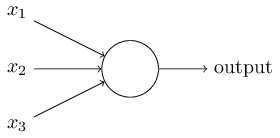
\includegraphics[width=.5\linewidth]{./img/erstesPerceptron}
	\mycaption{Perceptron - drei Eingabewerte}{dlnielsen}
	\label{fig:erstesPerceptron}
\end{figure}

Die Abbildung \ref{fig:erstesPerceptron} beschreibt ein einfaches Perceptron mit drei Eingabewerten. Genau wie die MP-Zelle verwendet dieses Modell einen Schwellwert $\theta$ um den letztendlichen Ausgabewert zu bestimmen, jedoch möchte ich hier noch einmal etwas genauer auf die Notation des Ganzen eingehen, da diese auch in späteren Abschnitten benötigt wird. 

\begin{equation} \label{eq:1}
g(\mathbf{z}) =\begin{cases}
	0 & \mbox{if } \mathbf{z} \leq \theta \\
    1 & \mbox{if } \mathbf{z} > \theta
  \end{cases}
\end{equation}

wobei gilt 

\begin{equation} \label{eq:vektorprod}
\mathbf{w} = \begin{bmatrix}
    w_{1}  \\
    \vdots \\
    w_{m}
\end{bmatrix}
\quad  \mathbf{x} = \begin{bmatrix}
    x_{1}  \\
    \vdots \\
    x_{m}
\end{bmatrix}
\end{equation}

\begin{equation}
\mathbf{z} =  w_1x_{1} + \dots + w_mx_{m} = \sum_{j=1}^{m} x_{j}w_{j} \\ = \mathbf{w}^T\mathbf{x}
\end{equation}

Sämtliche Gewichte und Eingabewerte können als Vektoren betrachtet werden. Die Summe der Produkte kann dadurch wiederum schlicht als \emph{Vektorpunktprodukt} verstanden werden (\ref{eq:vektorprod}).
